% =====================================================================
% BMED365: Lecture 1 Teaser — The Kiwi 3D Seed Segmentation Challenge
% =====================================================================
\documentclass[aspectratio=169, 10pt]{beamer}

\usepackage[utf8]{inputenc}
\usepackage[T1]{fontenc}
\usepackage[english]{babel}
\usepackage{graphicx}
\usepackage{booktabs}
\usepackage{amsmath}
\usepackage{xcolor}
\usepackage{hyperref}
\hypersetup{
    colorlinks=true,
    linkcolor=blue!70!black,
    urlcolor=blue!70!black
}

\usetheme{Madrid}
\usecolortheme{beaver}
\setbeamertemplate{navigation symbols}{}

\title[Kiwi 3D Challenge]{The Kiwi 3D Seed Challenge}
\subtitle{A 6-Week Red Thread in Computational Imaging, Modeling \& Semi-Verifiable AI}
\author[A. Lundervold (BMED365)]{Arvid Lundervold}
\institute[UiB \& MMIV]{Department of Biomedicine \& MMIV, University of Bergen\\BMED365 --- Spring 2027}
\date{Lecture 1 Teaser $\cdot$ Monday 4 January 2027}

\begin{document}

% ---------------------------------------------------------------------
% SLIDE 1: Title
% ---------------------------------------------------------------------
\begin{frame}
    \titlepage
\end{frame}

% ---------------------------------------------------------------------
% SLIDE 2: Live Poll & Dataset
% ---------------------------------------------------------------------
\begin{frame}{One Intact Kiwifruit, Three Deceptively Simple Questions}
    \begin{columns}[T,onlytextwidth]
        \column{0.47\textwidth}
        \centering
        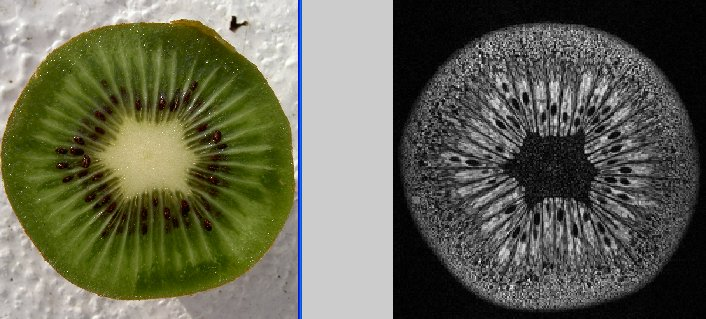
\includegraphics[width=\textwidth,height=0.66\textheight,keepaspectratio]{../assets/photo_mri_kiwi_20050219.jpg}
        \vspace{0.1cm}

        {\scriptsize Preclinical \textbf{7\,T Bruker Pharmascan} MRI (UiB, Feb 2005)\\
        $256 \times 256 \times 128$ voxels $\cdot$ $0.234 \times 0.234 \times 0.500\text{ mm}^3$}

        \column{0.50\textwidth}
        \begin{alertblock}{30-Second Classroom Poll}
            \textbf{1.} Roughly how many seeds ($N$) are inside this intact kiwifruit? \textit{(200? \ 600? \ 1,400? \ 4,000?)}\\[0.25em]
            \textbf{2.} What fraction of the fruit's 3D volume do the seeds occupy?\\[0.25em]
            \textbf{3.} \textbf{The Catch:} Nobody ever cut this 2005 fruit open to count the seeds. \textit{How can we verify if an AI or algorithm is right?}
        \end{alertblock}

        \vspace{0.15cm}
        \begin{itemize}
            \item \textbf{Zero medical jargon on Day 1:} Everyone knows what a kiwifruit looks like inside.
            \item \textbf{Real 3D MRI physics:} Anisotropic slices ($0.50\text{ mm} > 0.234\text{ mm}$), partial-volume blurring, and closely packed 3D instances.
        \end{itemize}
    \end{columns}
\end{frame}

% ---------------------------------------------------------------------
% SLIDE 3: Clinical Biomarker Analogy ("Lesion Load") & MRI Contrast
% ---------------------------------------------------------------------
\begin{frame}{Why a Kiwifruit in Biomedicine? Quantitative ``Lesion Load''}
    \begin{columns}[T,onlytextwidth]
        \column{0.55\textwidth}
        \textbf{Identical computational task in clinical neuroimaging:}
        \vspace{0.15cm}

        {\scriptsize
        \begin{tabular}{@{}p{0.42\textwidth}p{0.50\textwidth}@{}}
            \toprule
            \textbf{7\,T Kiwifruit MRI} & \textbf{Clinical / Biomedical Analogy} \\
            \midrule
            Whole fruit ($V_{\text{kiwi}} \approx 86\text{ cm}^3$) & Brain parenchyma (skull-stripped MRI) \\
            Dark 3D seeds ($N \approx \text{?}$) & MS plaques, cerebral microbleeds, micrometastases, or 3D cell nuclei \\
            Seed fraction $V_{\text{seeds}} / V_{\text{kiwi}}$ & \textbf{Quantitative ``Lesion Load''} \\
            Touching seeds in a chamber & Confluent vs.\ discrete focal lesions \\
            \bottomrule
        \end{tabular}
        }

        \vspace{0.25cm}
        \begin{block}{MRI Physics Twist: Contrast Inversion!}
            In an optical photo, the central core (\textit{columella}) is \textbf{bright white}. In $T_2$-weighted RARE MRI ($\text{TE}=63.9\text{ ms}$), dense fibrous core tissue has short $T_2$ and turns \textbf{dark} --- mimicking seeds!
        \end{block}

        \column{0.42\textwidth}
        \centering
        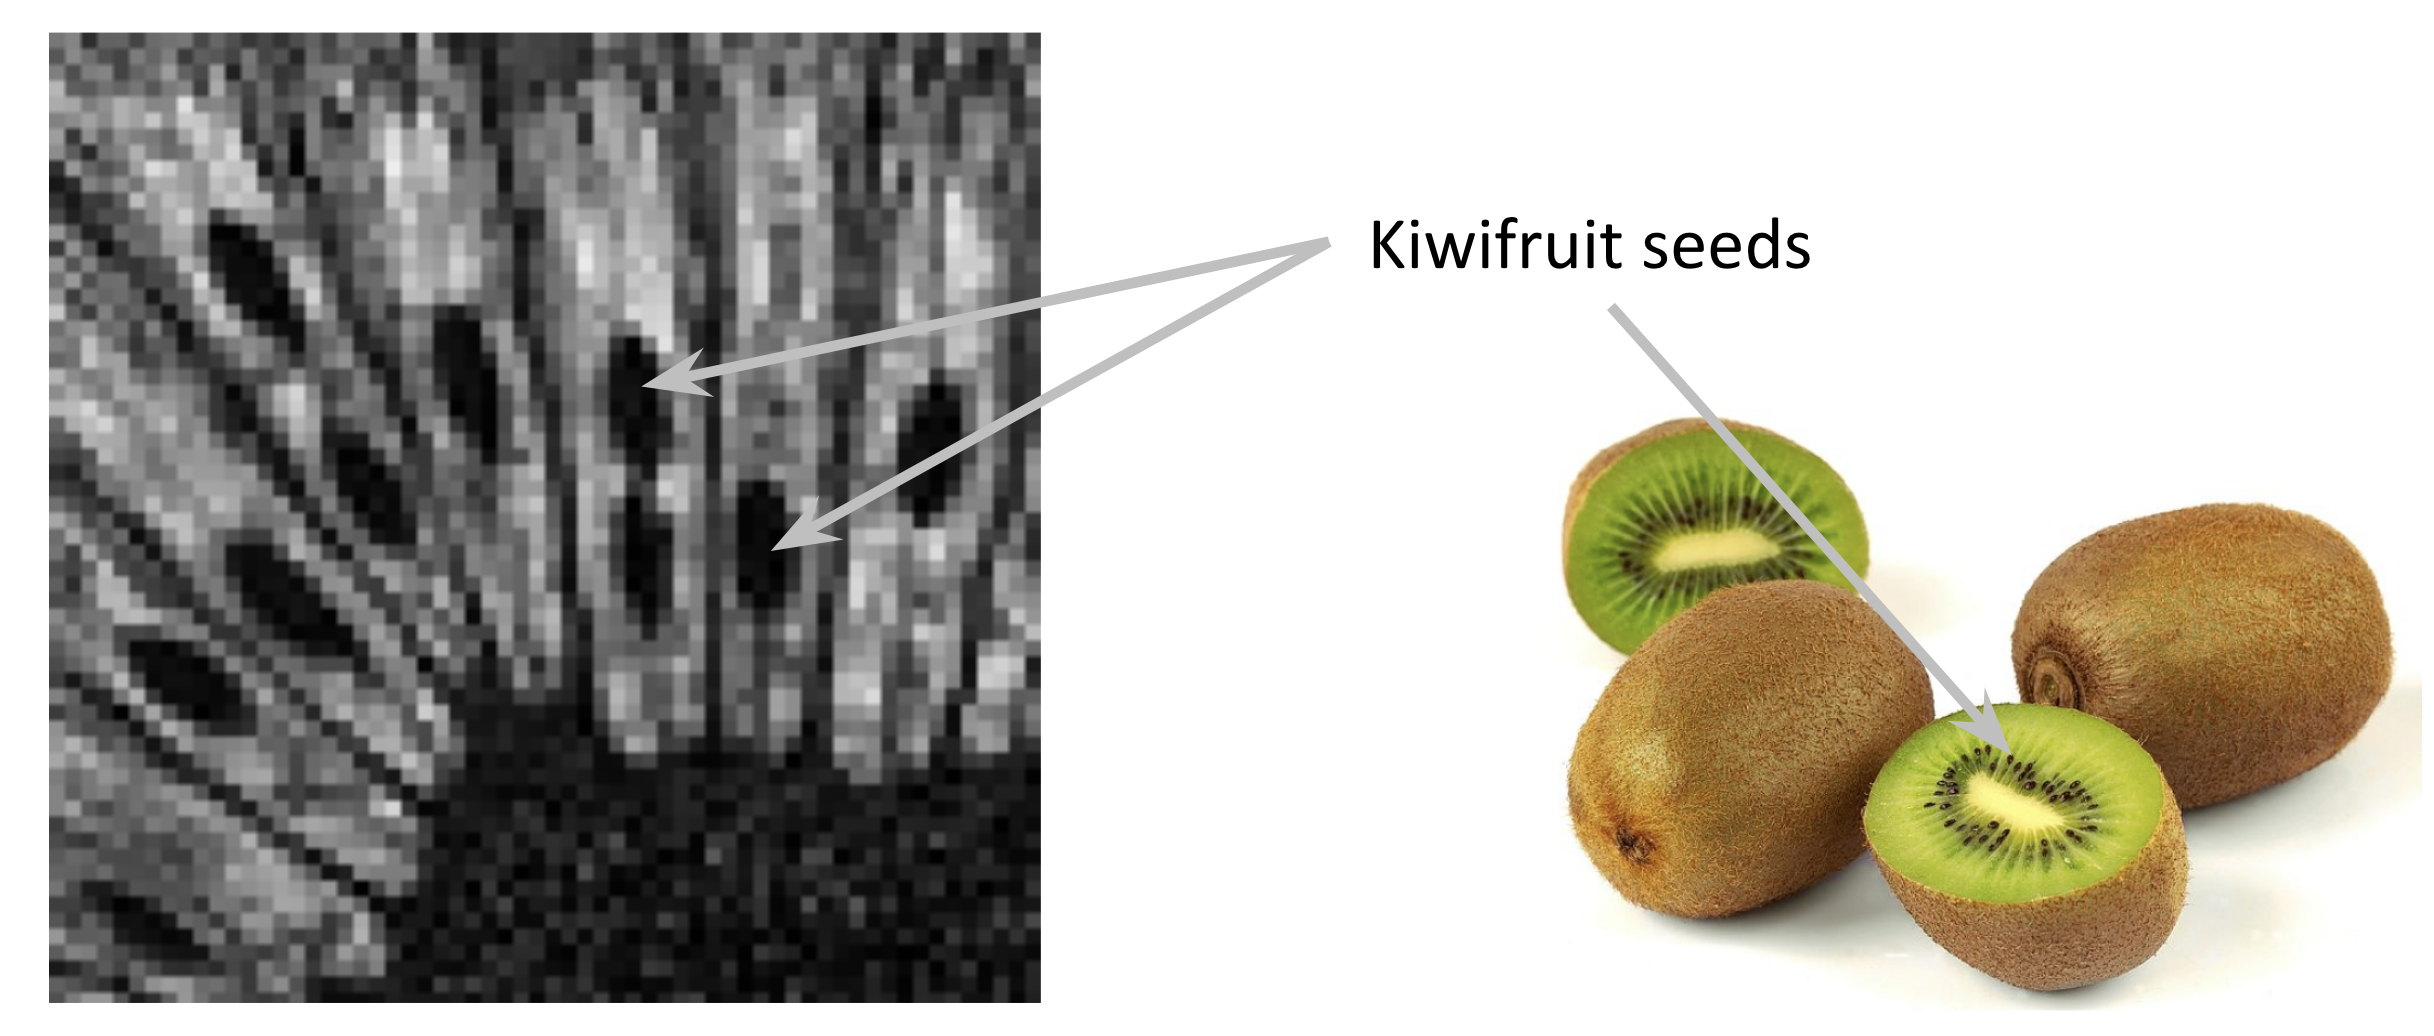
\includegraphics[width=\textwidth,height=0.72\textheight,keepaspectratio]{../assets/kiwi-seed-segmentation-task.png}
    \end{columns}
\end{frame}

% ---------------------------------------------------------------------
% SLIDE 4: Two Naive Day-1 Traps
% ---------------------------------------------------------------------
\begin{frame}{Two Day-1 Traps: Naive Thresholding vs.\ Raw Chatbot Counting}
    \centering
    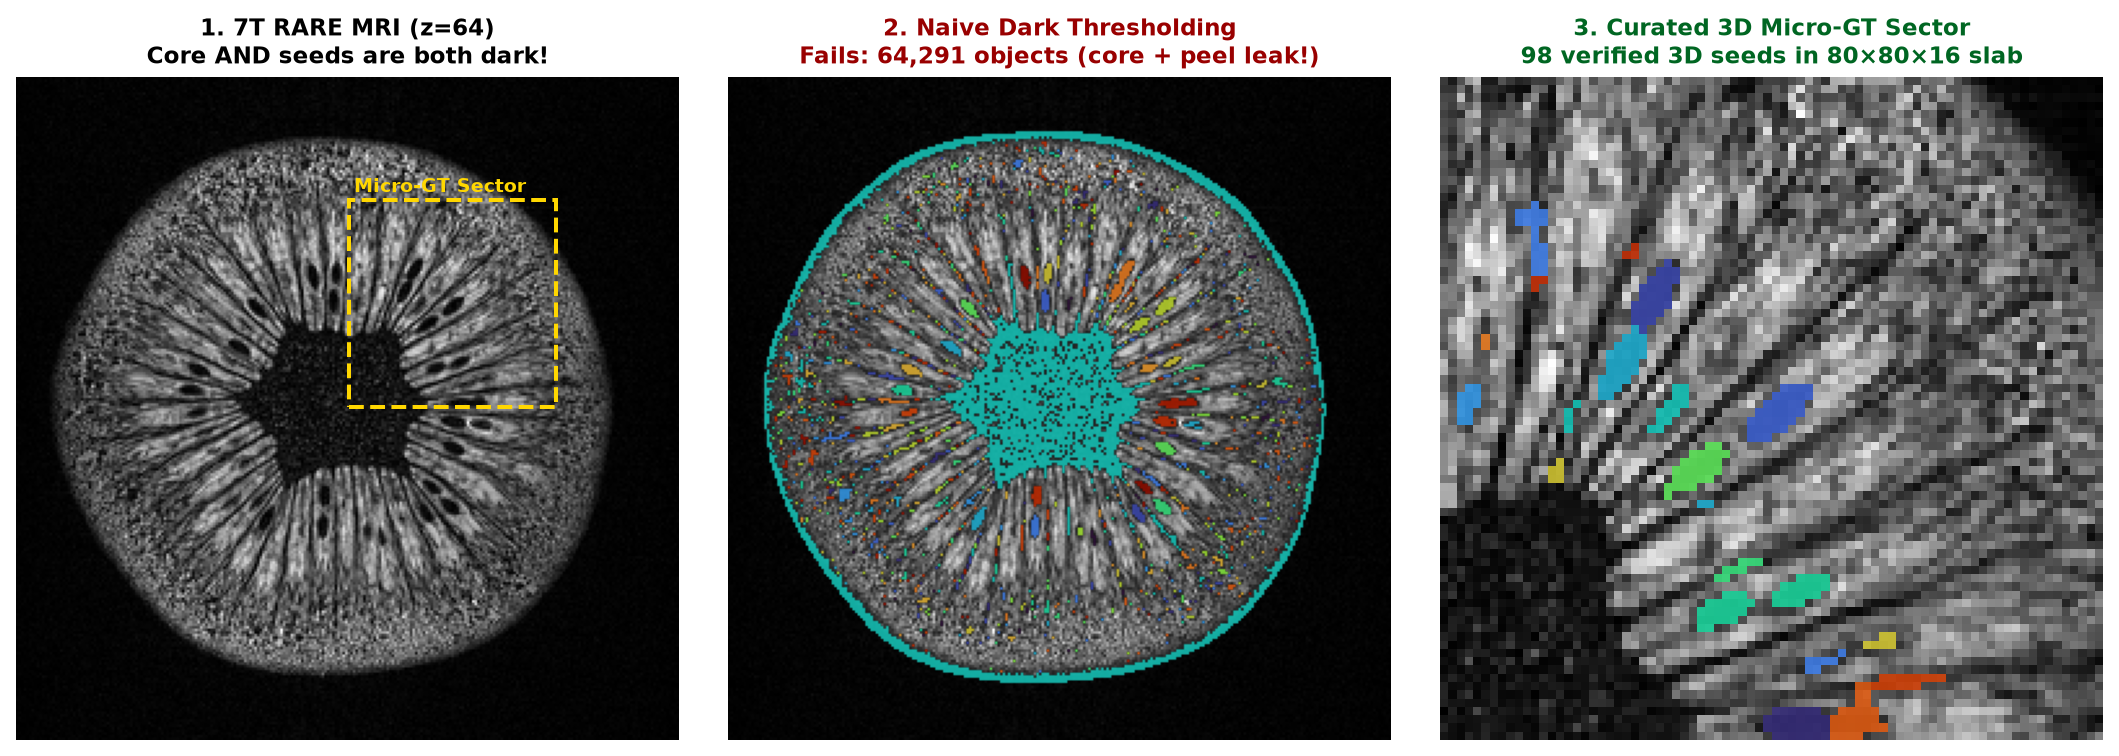
\includegraphics[width=0.95\textwidth,height=0.48\textheight,keepaspectratio]{../assets/kiwi_lecture1_teaser_card.png}

    \vspace{0.10cm}
    \begin{columns}[T,onlytextwidth]
        \column{0.48\textwidth}
        \begin{alertblock}{Trap 1: ``Just Threshold Dark Voxels''}
            \footnotesize Darkness $\neq$ seed! Thresholding leaks into the dark central core and outer peel, producing \textbf{64,291 fragments} + a giant $11{,}300\text{ mm}^3$ megablob.
        \end{alertblock}

        \column{0.48\textwidth}
        \begin{exampleblock}{Trap 2: ``Ask a Vision LLM to Count''}
            \footnotesize Multimodal chatbots output a fluent, confident integer on \texttt{kiwi\_064.png} --- yet hallucinate counts and ignore 128-slice 3D geometry. \textbf{Use AI to write \& verify 3D code!}
        \end{exampleblock}
    \end{columns}
\end{frame}

% ---------------------------------------------------------------------
% SLIDE 5: Historical Milestone & Semi-Verifiability
% ---------------------------------------------------------------------
\begin{frame}{Semi-Verifiability: Auditing Algorithms Without Complete Ground Truth}
    \begin{columns}[T,onlytextwidth]
        \column{0.43\textwidth}
        \centering
        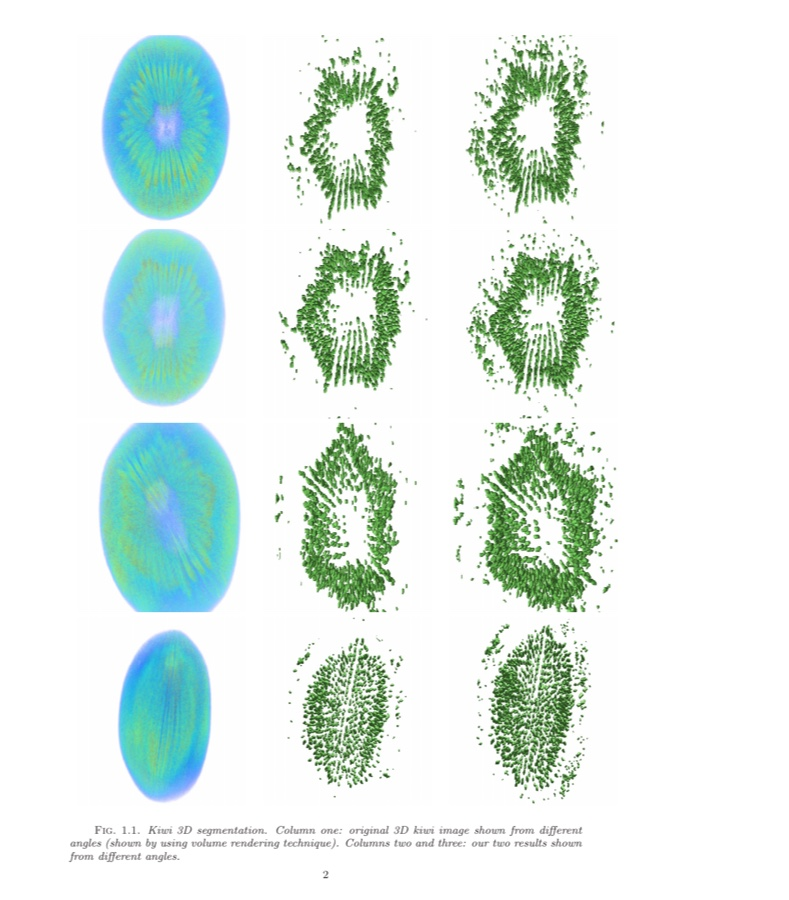
\includegraphics[width=\textwidth,height=0.58\textheight,keepaspectratio]{../assets/kiwi_3d_cai_chan_2012.jpg}
        \vspace{0.08cm}

        {\scriptsize \textbf{Dagstuhl / CUHK Milestone (2012):} 3D convex Mumford--Shah surfaces by X.~Cai \& R.\,H.~Chan.\\
        \textit{``Could you give us comments as to the quality of the segmentation?''}}

        \column{0.54\textwidth}
        \textbf{How our Lab 4 Verification Harness checks any method:}
        \vspace{0.1cm}
        \begin{enumerate}\footnotesize
            \item \textbf{Multi-Planar 3D Overlay:} Axial ($z=64$) + coronal ($y=128$) alignment across anisotropic slices.
            \item \textbf{Botanical Volume Prior:} Real \textit{Actinidia} seeds span $\mathbf{0.35\text{--}3.5\text{ mm}^3}$ ($\sim 13\text{--}127$ voxels).
            \item \textbf{Anatomical Zone Check:} Seeds sit in bright radial locules ($0.25 \le r/R \le 0.65$); $\sim 0\%$ in core or peel.
            \item \textbf{Synthetic 3D Injection:} Implant $K=25$ known synthetic seeds and verify sensitivity ($\pm 10\%$).
            \item \textbf{Curated 3D Micro-GT Sector ($80\times 80\times 16$):} 98 verified 3D seeds give objective \textbf{Precision, Recall, F1} \& bias-calibrated whole-fruit count ($\hat{N}_{\text{cal}} \approx 1{,}440$, lesion load $\approx 1.7\%$).
        \end{enumerate}
    \end{columns}
\end{frame}

% ---------------------------------------------------------------------
% SLIDE 6: The 6-Week Red Thread Across BMED365
% ---------------------------------------------------------------------
\begin{frame}{Your 6-Week Red Thread: Same 3D MRI, Evolving AI Paradigms}
    \centering
    {\scriptsize
    \begin{tabular}{@{}p{0.26\textwidth}p{0.37\textwidth}p{0.29\textwidth}@{}}
        \toprule
        \textbf{Course Module} & \textbf{Paradigm on the Kiwi MRI} & \textbf{Key Question} \\
        \midrule
        \textbf{Quick Start \& Lab 0} (Wk 1--2) & Voxel features, top-hat filters, K-means / AutoML & What separates seeds from core/peel? \\
        \textbf{Lab 1: Networks} (Wk 1) & 3D spatial centroid graph in radial chambers & Can anatomy spot outliers \& merges? \\
        \textbf{Lab 2: Deep Learning} (Wk 2) & 2D/3D U-Net, StarDist, Cellpose, MedSAM / SAM\,2 & Do foundation models generalize? \\
        \textbf{Lab 3: GenAI \& Agents} (Wk 3) & Prompted vs.\ verifier-guided coding agents & Can an agent optimize our harness? \\
        \textbf{Lab 4: Comp.\ Imaging} (Wk 6) & \textbf{Live Comparative Showdown (Notebooks 01--03)} & Which paradigm wins --- and \textit{why}? \\
        \bottomrule
    \end{tabular}
    }

    \vspace{0.3cm}
    \begin{block}{Explore Anytime \& Optional Block 2 Individual Project}
        \footnotesize
        \begin{itemize}
            \item \textbf{Repository \& 1-Click Colab Notebooks:} \href{https://github.com/arvidl/BMED365-2027/tree/main/Lab4-Comp-Imag/Kiwi-challenge}{\texttt{Lab4-Comp-Imag/Kiwi-challenge}} (\texttt{01}, \texttt{02}, and \texttt{03} + curated 3D Micro-GT NIfTI for ITK-SNAP / 3D Slicer).
            \item \textbf{Individual Project Idea (Weeks 4--6):} Benchmark classical, foundation-model (\texttt{SAM\,2} / \texttt{Cellpose}), or agentic 3D segmentation pipelines on this self-contained 7\,T dataset!
        \end{itemize}
    \end{block}
\end{frame}

\end{document}
